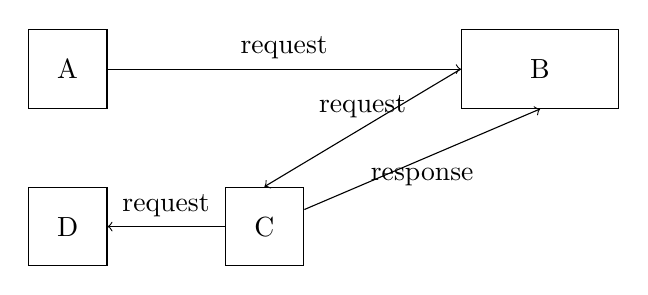
\begin{tikzpicture}
  \node (tabs) [rectangle, draw, minimum height=1cm, minimum width=1cm] at (0, 1) {A};
  \node (editor) [rectangle, draw, minimum height=1cm, minimum width=2cm] at (6, 1) {B};
  \node (fsa) [rectangle, draw, minimum height=1cm, minimum width=1cm] at (2.5, -1) {C};
  \node (cache) [rectangle, draw, minimum height=1cm, minimum width=1cm] at (0, -1) {D};

  \draw[->] (tabs) to node[midway, above] {request} (editor);
  \draw[->] (editor.west) to node[midway, above] {request} (fsa.north);
  \draw[->] (fsa) to node[midway, below] {response} (editor.south);
  \draw[->] (fsa) to node[midway, above] {request} (cache);
\end{tikzpicture}
